\documentclass[letterpaper]{article}
\usepackage[margin=1in]{geometry}
\usepackage[utf8]{inputenc}
\usepackage{textcomp}
\usepackage{amssymb}
\usepackage{natbib}
\usepackage{graphicx}
\usepackage{gensymb}
\usepackage{amsthm, amsmath, mathtools}
\usepackage[dvipsnames]{xcolor}
\usepackage{enumerate}
\usepackage{mdframed}
\usepackage[most]{tcolorbox}
\usepackage{csquotes}
% https://tex.stackexchange.com/questions/13506/how-to-continue-the-framed-text-box-on-multiple-pages

\tcbuselibrary{theorems}

\newcommand{\R}{\mathbb{R}}
\newcommand{\Z}{\mathbb{Z}}
\newcommand{\N}{\mathbb{N}}
\newcommand{\Q}{\mathbb{Q}}
\newcommand{\C}{\mathbb{C}}
\newcommand{\code}[1]{\texttt{#1}}
\newcommand{\mdiamond}{$\diamondsuit$}
\newcommand{\PowerSet}{\mathcal{P}}
\newcommand{\Mod}[1]{\ (\mathrm{mod}\ #1)}
\DeclareMathOperator{\lcm}{lcm}

%\newtheorem*{theorem}{Theorem}
%\newtheorem*{definition}{Definition}
%\newtheorem*{corollary}{Corollary}
%\newtheorem*{lemma}{Lemma}
\newtheorem*{proposition}{Proposition}


\newtcbtheorem[number within=section]{theorem}{Theorem}
{colback=green!5,colframe=green!35!black,fonttitle=\bfseries}{th}

\newtcbtheorem[number within=section]{definition}{Definition}
{colback=blue!5,colframe=blue!35!black,fonttitle=\bfseries}{def}

\newtcbtheorem[number within=section]{corollary}{Corollary}
{colback=yellow!5,colframe=yellow!35!black,fonttitle=\bfseries}{cor}

\newtcbtheorem[number within=section]{lemma}{Lemma}
{colback=red!5,colframe=red!35!black,fonttitle=\bfseries}{lem}

\newtcbtheorem[number within=section]{example}{Example}
{colback=white!5,colframe=white!35!black,fonttitle=\bfseries}{def}

\newtcbtheorem[number within=section]{note}{Important Note}{
        enhanced,
        sharp corners,
        attach boxed title to top left={
            xshift=-1mm,
            yshift=-5mm,
            yshifttext=-1mm
        },
        top=1.5em,
        colback=white,
        colframe=black,
        fonttitle=\bfseries,
        boxed title style={
            sharp corners,
            size=small,
            colback=red!75!black,
            colframe=red!75!black,
        } 
    }{impnote}
\usepackage[utf8]{inputenc}
\usepackage[english]{babel}
\usepackage{fancyhdr}
\usepackage[hidelinks]{hyperref}

\pagestyle{fancy}
\fancyhf{}
\rhead{Math 170B}
\chead{Friday, May 26, 2023}
\lhead{Lecture 24}
\rfoot{\thepage}

\setlength{\parindent}{0pt}

\begin{document}
\section{Nelder-Mead Simplex Method (Section 11.5)}
As usual, our goal is to minimize a function $f(x): \R^n \to \R$. This method is a direct search method, but does not require a derivative of the function $f$ and doesn't make use of any line searches. This method is versatile, but may be restricted to smaller problems\footnote{In other words, for a small $n$.}. 

\bigskip 

Before beginning the calculations, we assign values to three parameters, $\alpha = 1$, $\beta = \frac{1}{2}$, and $\gamma = 1$. The values described here are the default values. In each step of this method, we'll have a set of $n + 1$ points $x^{(i)} \in \R^n$,  
\[\{x^{(0)}, x^{(1)}, \hdots, x^{(n)}\}.\]
Note that the set of vectors should be in general position in $\R^n$; that is, \textbf{the set of $n$ points $x^{(i)} - x^{(0)}$ for $1 \leq i \leq n$ is linearly independent}.

\begin{mdframed}
    (Example.) Suppose we're in $\R^2$. We have three points in our set, $x^{(0)} \in \R^2$, $x^{(1)} \in \R^2$, and $x^{(2)} \in \R^2$. This gives us 
    \begin{center}
        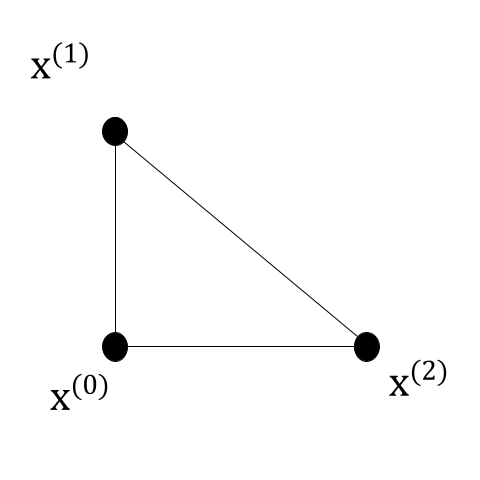
\includegraphics[scale=0.4]{../assets/triangle_simplex.png}
    \end{center}
    Here, we can consider $x^{(1)}$ and $x^{(2)}$ to be linearly independent, and $x^{(0)}$ is at the origin. By connecting these points with a border, we create a convex hull with the set of points. This convex hull represents a simplex. 
\end{mdframed}
We want to reorder/relabel the points so that 
\[f(x^{(0)}) \geq f(x^{(1)}) \geq \hdots \geq f(x^{(n)}).\]

\subsection{Operations on the Search Space}
Based on the ordering, the search space will be modified in order to find the desirable points. As one might expect, $f(x^{(0)})$ is the worst and $f(x^{(n)})$ is the best. Some operations to explore the search space include 
\begin{itemize}
    \item \textbf{Centroid:} $u = \frac{1}{n} \sum_{i = 1}^{n} x^{(i)}$. This is the centroid of the face of the current simplex opposite the worst vertex, $x^{(0)}$. 
    \item \textbf{Reflection:} $v = (1 + \alpha)u - \alpha x^{(0)} - \alpha x^{(0)}$
    \item \textbf{Expansion:} $w = (1 + \gamma)v - \gamma u$. This checks if $v$ was improving the best function value, whether $w$ would improve it even more. 
    \item \textbf{Reduction:} $w' = \beta x^{(0)} + (1 - \beta) u$. 
\end{itemize}
\begin{mdframed}
    (Example.) If we have $x^{(0)} = \begin{bmatrix}
        0 \\ 0 
    \end{bmatrix}$, $x^{(1)} = \begin{bmatrix}
        0 \\ 1
    \end{bmatrix}$, and $x^{(2)} = \begin{bmatrix}
        1 \\ 0
    \end{bmatrix}$, then we know $n = 2$ and 
    \[u = \frac{1}{n} \sum_{i = 1}^{n} x^{(i)} = \frac{1}{2} \sum_{i = 1}^{2} x^{(i)} = \frac{1}{2} \left(\begin{bmatrix}
        0 \\ 1
    \end{bmatrix} + \begin{bmatrix}
        1 \\ 0
    \end{bmatrix}\right) = \frac{1}{2}\begin{bmatrix}
        1 \\ 1
    \end{bmatrix}.\]
\end{mdframed}

Roughly speaking, these operations look like 
\begin{center}
    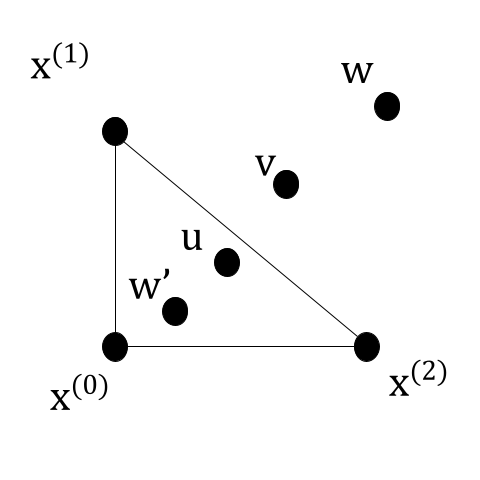
\includegraphics[scale=0.35]{../assets/triangle_simplex4.png}
\end{center}
In particular, part of the check we need to do is whether $f(v) < f(x^{(n)})$. If this is the case, we can compute $w$ (the expansion) and see whether this expansion is further beneficial. In particular, we want to see if $f(w) < f(x^{(n)})$; if this is the case, then we can set $x^{(0)} \gets w$ and $f(x^{(0)}) \gets f(w)$. Otherwise, we can set $x^{(0)} \gets v$ and $f(x^{(0)}) \gets f(v)$. 


\subsection{Desirable Stopping Condition}
A desirable stopping condition is the \textbf{relative flatness}; that is, 
\[\frac{f(x^{(0)}) - f(x^{(n)})}{\max\{|f(x^{(0)})| + |f(x^{(n)})|, 1\}}.\]
Note that we have the maximum condition in the denominator to avoid dividing by 0. So, we would stop if the ``relative flatness'' is sufficiently small enough.

\subsection{Algorithm}
The implementation we'll use does not reorder all the functions, as this is an expensive process (sorting in general is expensive). Instead, we only swap the relative indices. With this said, our function takes the following inputs: 
\begin{itemize}
    \item $f$, the function to evaluate. 
    \item $\{x^{(0)}, x^{(1)}, \hdots, x^{(n)}\}$, the set of candidate points. 
    \item $\epsilon$, the tolerance. 
    \item $M$, the maximum number of iterations. 
    \item $\alpha, \beta, \gamma$, the three parameters mentioned earlier.
\end{itemize} 
\begin{algorithm}[H]
    \caption{Nelder-Mead Simplex Method}
    \begin{algorithmic}[1]
        \Function{NelderMeadSimplex}{$f, \{x^{(i)}\}, \epsilon, M, \alpha, \beta, \gamma$}
            \For{$i \gets 1$ to $n + 1$} \Comment{Corresponds to constructing simplex by defining values at each vertex.}
                \State $F(i) = f(x^{(i - 1)})$ \Comment{$F$ is the vector of all function values.}
                \State $X(:, i) = x^{(i - 1)}$ \Comment{Storing the points into the matrix.}
            \EndFor 
            \State $(f_n, i_n) = \min(F)$ % L1
            \State $(f_0, f_1, i_0, i_1) = \max_{2}(F)$ % L2
            \State $o \gets [1]_{n \times 1}$ \Comment{$n \times 1$ vector of 1's.}
            \State $k \gets 0$
            \While{$(f_{0} - f_{n}) / (\max\{|f_{0}| + |f_{1}|, 1\}) \geq \epsilon$ and $k < M$}
                \State $u \gets \frac{1}{n}\sum_{\ell = 1}^{n} x^{(\ell)}$
                \State $v \gets (1 + \alpha) u - \alpha X(:, i_0)$
                \State $f_v = f(v)$
                \If{$f_v < f_n$}
                    \State $w \gets (1 + \gamma) v - \gamma u$
                    \State $f_w \gets f(w)$
                    \If{$f_w < f_n$}
                        \State $X(:, i_0) \gets w$
                        \State $f_0 \gets f_w$
                    \Else 
                        \State $X(:, i_0) \gets v$
                        \State $f_0 \gets f_v$
                    \EndIf    
                \Else 
                    \If{$f_v \leq f_1$}
                        \State $X(:, i_0) \gets v$
                        \State $f_0 \gets f_v$
                    \Else 
                        \State $b \gets f_0$
                        \If{$f_v \leq f_0$}
                            \State $X(:, i_0) \gets v$
                            \State $f_0 \gets f_v$
                        \EndIf 

                        \State $w \gets \beta X(:, i_0) + (1 - \beta) u$
                        \State $f_w \gets f(w)$

                        \If{$f_w \leq b$}
                            \State $X(:, i_0) \gets w$
                            \State $f_0 \gets f_w$
                        \Else 
                            \For{$i \gets 1$ to $n + 1$}
                                \If{$i \neq i_n$}
                                    \State $X(:, i) \gets \frac{1}{2} (X(:, i) + X(i, i_n))$
                                    \State $F(i) \gets f(X(:, i))$
                                    \State \textbf{break}
                                \EndIf 
                            \EndFor 
                        \EndIf 
                    \EndIf 
                \EndIf 

                \State $(f_n, i_n) \gets \min(F)$
                \State $(f_0, f_1, i_0, f_1) \gets \max_{2}(F)$
                \State $k \gets k + 1$
            \EndWhile 
        \EndFunction 
    \end{algorithmic}
\end{algorithm}
A few notes: 
\begin{itemize}
    \item In line 6, we're computing the index of the minimum point. So, $f_n$ is the smallest function value and $i_n$ is minimum index of said function value. % L1
    \item In line 7, we're finding the two largest function values $f_0, f_1$ and the corresponding indices $i_0, i_1$. Here, $\max_{k}$ means to find the $k$ highest elements. % L2
\end{itemize}

\end{document}